\begin{figure}[htbp]
\centering 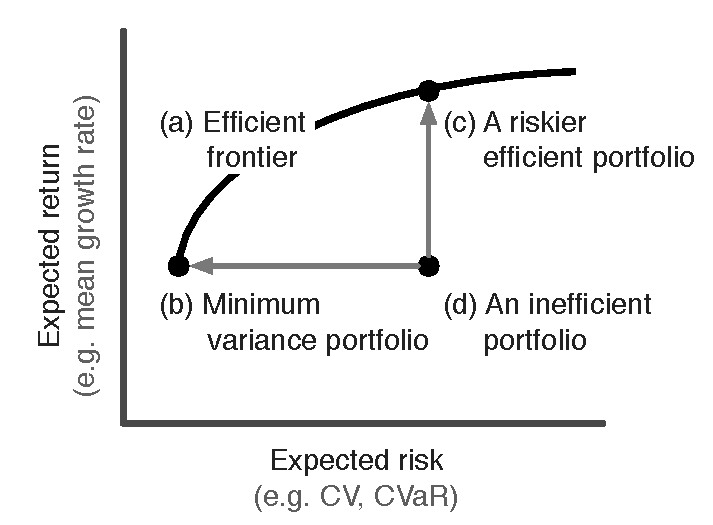
\includegraphics[width=3.5in]{efficient-frontier-fig.pdf}
\caption{An introduction to Modern Portfolio Theory mean-variance
  optimization. In finance, portfolios are formed by choosing how much to
  invest in various assets. Modern Portfolio Theory focuses on identifying the
  set of portfolios that optimizes the trade-off between expected return
  (`mean') and expected risk (`variance'). \textbf{(a)} The efficient frontier
  represents a set of portfolios that maximize expected return for a level of
  expected risk. A manager would choose a portfolio on the efficient frontier,
  but the relative position would depend on risk tolerance. \textbf{(b)} The
  minimum variance portfolio achieves the lowest expected risk; the remaining
  risk is said to be undiversifiable. \textbf{(c)} A risker, but still
  efficient portfolio. \textbf{(d)} An example inefficient portfolio, which
  has a lower expected return than (c) and greater expected risk than (b).
  Adapted from \citet{hoekstra2012}.} \label{fig:mpt}
\end{figure}

\clearpage

\begin{figure}[htbp]
\centering 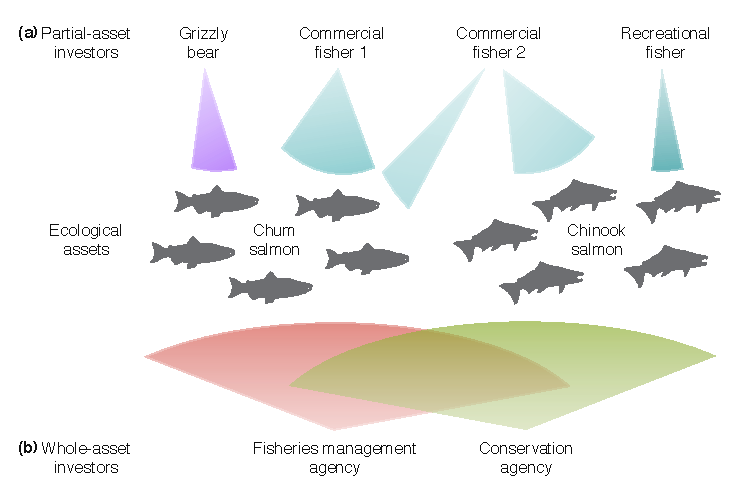
\includegraphics[width=5in]{salmon-portfolios.pdf} \caption{There
  are multiple ways of investing in ecological portfolios. In this example,
  investors are shown along the top and bottom and ecological assets are shown
  in the middle (populations of chum salmon, \textit{Oncorhynchus keta}, and
  Chinook salmon, \textit{Oncorhynchus tshawytscha}). The shaded arcs indicate
  investment. \textbf{(a)} Partial-asset investors invest by removing portions
  of the salmon populations --- the salmon that commercial fisher 1 removes are
  unavailable for the grizzly bear. These investors can often change their
  investment with ease. For example, commercial fisher 2 could decide to fish
  more Chinook and less chum salmon. Most financial portfolio theory is
  developed around this paradigm. \textbf{(b)} Whole-asset investors invest in
  entire populations. These investors can share assets but may have different
  goals for their portfolio. They can adjust their investment by managing
  properties of the population itself. For example, the fisheries management
  agency could reduce fishing of chum salmon to allow the population to grow.
  The conservation agency could fund habitat restoration for Chinook salmon to
  increase carrying capacity and expand their investment.}
\label{fig:salmonport}
\end{figure}

\begin{figure}[htbp]
\centering
%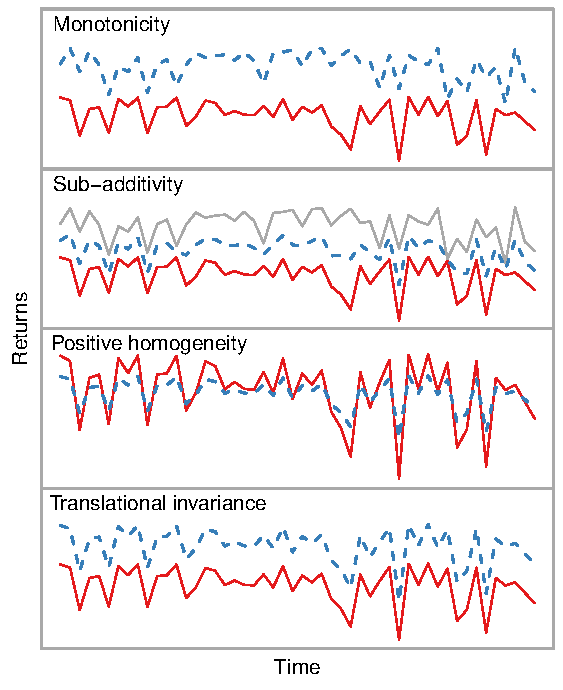
\includegraphics[width=2.6in]{coherence-axioms.pdf}
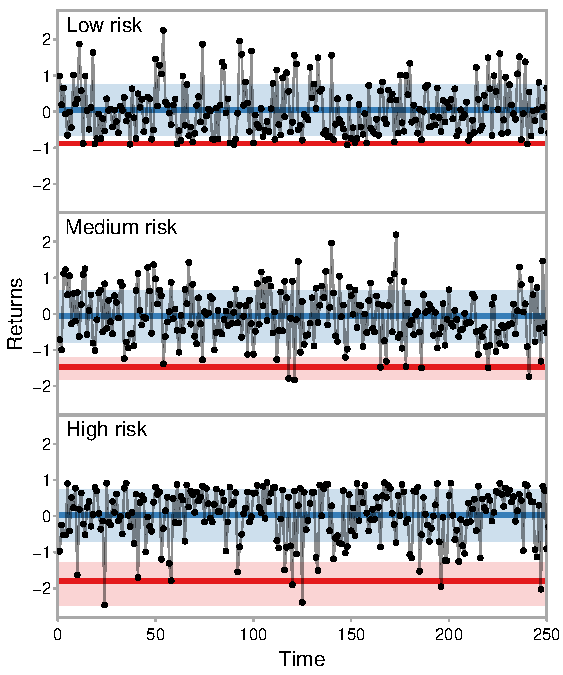
\includegraphics[height=3.0in]{skewness-abundance.pdf}
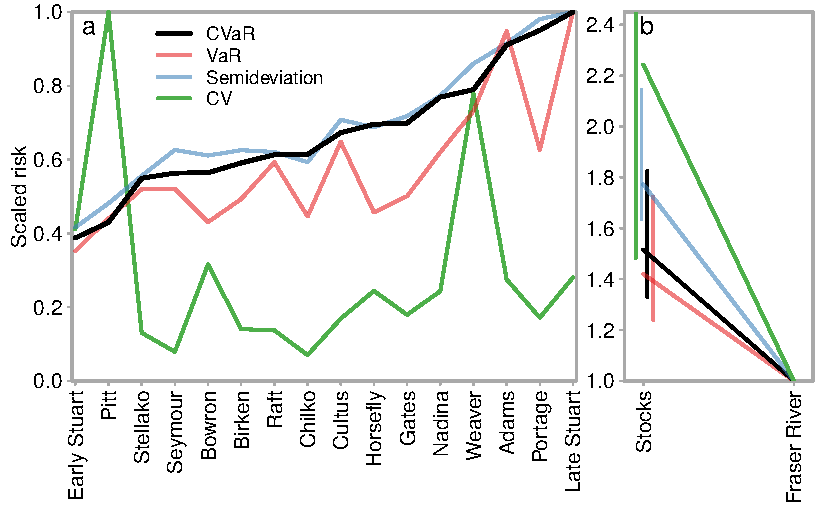
\includegraphics[height=2.0in]{compare-risk-and-portfolio-scale.pdf} \caption{
  Symmetric vs.\ downside risk measures. \textbf{(Left panel)} An illustration
  of three systems with the same symmetric variability but different levels of
  downside risk. The y-axis denotes rate of change of abundance or biomass
  (``returns'' in financial terminology). The dark blue line represents the
  mean and the blue shaded region represents $\pm$ one standard deviation --- a
  measure that does not account for the asymmetric property of risk. The red
  line represents the 95\% CVaR (conditional value at risk) and the red shaded
  region represents the region below the 95\% VaR (value at risk). CVaR and VaR
  are both downside risk measures that accurately identify higher risk systems.
  \textbf{(Right panel)} \textbf{(a)} Symmetric and downside risk metrics
  applied to annual returns of sockeye salmon stocks in the Fraser River (data
  from \citeauthor{dorner2008} \citeyear{dorner2008}). Stocks are ordered by
  increased CVaR. Symmetric (CV) and asymmetric (all other) risk metrics differ
  considerably in their rank order of risk for the different stocks.
  \textbf{(b)} The portfolio effect calculated for the same salmon stocks using
  the four risk metrics. Sloped lines at the stock level represent the mean
  portfolio effect and the vertical segments show the interquartile range.}
\label{fig:risk}
\end{figure}
